\documentclass[12pt]{article}

\usepackage{sbc-template}
\usepackage{graphicx,url}
\usepackage[utf8]{inputenc}
\usepackage[brazil]{babel}
\usepackage{booktabs}
\usepackage{microtype}

\sloppy

\title{Inferência Textual em Português \emph{Zero-Shot}:\\
Especialização Linguística \emph{vs.} Raciocínio Explícito\\
em Modelos de Linguagem Compactos}

\author{Gabriel Silvestre Mancini\inst{1} \and Marcos Lopes\inst{1}}

\address{Programa de Educação Continuada em Engenharia (PECE)\\
  Escola Politécnica -- Universidade de São Paulo (USP)\\
  Av. Prof. Luciano Gualberto, trav. 3, n. 380 -- 05508-010 -- São Paulo -- SP -- Brasil
  \email{gabrielsmancini@gmail.com, marcoslopes@usp.br}
}

\begin{document}

\maketitle

\begin{abstract}
This work investigates the inferential capabilities of small and medium-sized
language models (up to 9B parameters) on Natural Language Inference (NLI) in
Brazilian Portuguese under a strictly zero-shot regime. Grounded in the formal
semantic definition of entailment as truth-condition preservation~\cite{Ferreira2019}, a deductive relation in Peirce's tripartite classification~\cite{peirce_cp2},
we compare Portuguese-specialized models (Sabiá, Bode, Gaia) with recent
multilingual models that incorporate explicit reasoning and knowledge distillation
(Qwen3, Gemma~2, Ministral~3) on ASSIN~2 and on a controlled synthetic dataset
grounded in lexical inclusion (hyponymy/hyperonymy). Results show that explicit
reasoning and distillation are more decisive than monolingual adaptation alone,
and that high accuracy on ASSIN~2 may overestimate inferential competence by
conflating inductive distributional similarity with deductive truth-condition
preservation.
\end{abstract}

\begin{resumo}
Este trabalho investiga a capacidade inferencial de modelos de linguagem de
pequeno e médio porte (até 9B de parâmetros) na tarefa de Inferência em
Linguagem Natural (NLI) em português brasileiro, em regime estritamente
\emph{zero-shot}. Partindo da definição formal de acarretamento como
preservação de condições de verdade~\cite{Ferreira2019}, uma relação
dedutiva na classificação peirceana~\cite{peirce_cp2}, comparamos modelos
especializados em português (Sabiá, Bode, Gaia) com modelos multilíngues
equipados com mecanismos explícitos de raciocínio e destilação de conhecimento
(Qwen3, Gemma~2, Ministral~3) no ASSIN~2 e em um \emph{dataset} sintético
controlado, fundamentado em acarretamento por inclusão lexical
(hiponímia/hiperonímia). Os resultados indicam que raciocínio explícito e
destilação são mais decisivos do que adaptação monolíngue isolada, e que
acurácia elevada no ASSIN~2 pode superestimar a competência inferencial ao
confundir similaridade distribucional indutiva com preservação dedutiva de
condições de verdade.
\end{resumo}

\section{Introdução}

Na semântica formal, o acarretamento é definido como uma relação de preservação
de condições de verdade entre sentenças: $S_1$ acarreta $S_2$ quando, em toda
situação possível em que $S_1$ é verdadeira, $S_2$ também o
é~\cite{Ferreira2019}. Essa noção lógica estrita, que na tipologia peirceana
corresponde à \emph{dedução}, o único tipo de inferência que preserva verdade
necessariamente~\cite{peirce_cp2}, distingue-se radicalmente da similaridade
semântica distribucional, processo \emph{indutivo} que mede graus de semelhança
léxico-contextual a partir de padrões observados nos dados de treinamento.

É precisamente essa dissociação entre relação dedutiva (acarretamento) e
reconhecimento indutivo (similaridade) que torna o Reconhecimento de Inferência
Textual (NLI) em português um desafio em aberto, especialmente para modelos
compactos (até 9B de parâmetros) em regime estritamente \emph{zero-shot}. Dois
paradigmas concorrentes disputam esse espaço: modelos \emph{especialistas} em
português, via pré-treinamento contínuo ou ajuste fino instrucional (Sabiá
\cite{Pires_2023_sabia}, Bode \cite{bode2024}, Gaia
\cite{gaia-gemma-3-4b-2025}), e modelos \emph{generalistas} multilíngues com
mecanismos explícitos de raciocínio e destilação de conhecimento (Qwen3
\cite{yang2025qwen3technicalreport}, Ministral~3 \cite{liu2026ministral3},
Gemma \cite{gemmateam2024gemma2improvingopen}).

Este trabalho contribui em duas frentes. Primeiro, avalia comparativamente
11~LLMs no \emph{benchmark} ASSIN~2 \cite{real2020assin} em regime
\emph{zero-shot}. Segundo, introduz um \emph{dataset} sintético controlado,
fundamentado em acarretamento por inclusão lexical (hiponímia/hiperonímia) e
alinhado à definição formal de Ferreira~\cite{Ferreira2019}, para mitigar
efeitos de familiaridade prévia dos modelos com o \emph{benchmark} e isolar
competência inferencial genuína.

\section{Fundamentação e Trabalhos Relacionados}

\subsection{Inferência lógica: dedução, indução e abdução}

Peirce classifica as inferências lógicas em três tipos com estruturas
silogísticas distintas~\cite{peirce_cp2,peirce_cp5}. A \textbf{dedução} parte
de uma regra geral e de um caso para uma conclusão necessariamente verdadeira, é o único tipo em que a verdade das premissas \emph{garante} a verdade da
conclusão. A \textbf{indução} generaliza a partir de casos observados para uma
regra probabilística: opera ampliativamente e está sujeita à revisão pela
experiência. A \textbf{abdução} gera hipóteses explicativas para fatos
surpreendentes, produzindo conclusões apenas prováveis.

Essa tipologia é diretamente relevante para a tarefa de NLI. O acarretamento
semântico, relação que NLI pretende reconhecer, é por definição dedutivo:
$S_1 \Rightarrow S_2$ significa que não existe situação em que $S_1$ seja
verdadeira e $S_2$ falsa~\cite{Ferreira2019}. Modelos de linguagem, porém, são
treinados por estimativa de máxima verossimilhança, um processo
fundamentalmente \emph{indutivo}: aprendem regularidades estatísticas dos dados
de treinamento e generalizam a partir delas. A questão empírica central deste
trabalho é, portanto, se o treinamento indutivo, com ou sem especialização
em português, é capaz de produzir comportamento dedutivo robusto na
verificação de condições de verdade.

\subsection{Acarretamento semântico e inclusão lexical}

Na semântica formal, a operacionalização linguística mais direta do
acarretamento é a \emph{inclusão de sentido}~\cite{Ferreira2019}: se um
predicado contém um hipônimo, a hipótese obtida pela substituição desse
hipônimo por seu hiperônimo é necessariamente acarretada. Por exemplo,
\emph{O lateral-esquerdo sofreu a falta} acarreta \emph{O jogador sofreu a
falta} porque o conjunto de situações em que um lateral-esquerdo sofre uma
falta está contido no conjunto de situações em que um jogador sofre uma falta.
Essa relação é estritamente semântica: independe de implicaturas
conversacionais, pressuposições ou conhecimento enciclopédico extralinguístico.

A distinção entre acarretamento (relação lógica, dedutiva, baseada em
condições de verdade) e similaridade semântica distribucional (grau de
semelhança léxico-contextual, inferida indutivamente) é central para
interpretar tanto o \emph{design} dos \emph{benchmarks} quanto o comportamento
dos modelos avaliados.

\subsection{Benchmarks de NLI em português}

Os principais recursos para NLI em português são o SICK-BR~\cite{real18},
adaptação do corpus SICK do SemEval-2014 para o português brasileiro, e o
ASSIN~2~\cite{real2020assin}. O ASSIN~2 representa um avanço metodológico
importante ao adotar classificação binária (acarretamento \emph{vs.}
não-acarretamento) com sentenças simples extraídas do SICK-BR, reduzindo
complexidades sintáticas e discursivas que dificultavam a avaliação controlada
do raciocínio semântico.

No espectro supervisionado, o BERTimbau~\cite{bert-models} com \emph{fine-tuning}
no ASSIN~2 estabeleceu o estado da arte com acurácia próxima a 0,90. Em
contraste, \cite{stil} demonstraram que heurísticas simples, sobreposição
lexical, detecção de negação e diferença de comprimento entre premissa e
hipótese, atingem F1~$\approx$~0,71, evidenciando vieses estruturais no
\emph{benchmark} que permitem desempenho competitivo sem inferência semântica
profunda. Esse resultado levanta a hipótese de que parte do desempenho dos
modelos supervisados decorre de exploração de regularidades do \emph{dataset}
e não necessariamente de modelagem explícita de inferência lógica.

O intervalo entre o piso heurístico (0,71) e o teto supervisionado (0,90)
define o espaço no qual posicionamos a avaliação dos LLMs \emph{zero-shot}.

\subsection{Modelos compactos: especialização \emph{vs.} raciocínio}

Duas vertentes recentes competem no campo dos LLMs compactos. A primeira aposta
em \textbf{especialização linguística}: o Sabiá~\cite{Pires_2023_sabia} aplica
pré-treinamento contínuo de LLaMA sobre corpus em português (ClueWeb~22); o
Bode~\cite{bode2024} usa ajuste fino com LoRA em instruções traduzidas (Alpaca);
o Gaia~\cite{gaia-gemma-3-4b-2025} combina pré-treinamento contínuo (13B tokens
em português) com \emph{weight merging} para restaurar capacidade instrucional.

A segunda aposta em \textbf{raciocínio explícito e destilação}: o
Qwen3~\cite{yang2025qwen3technicalreport} integra \emph{thinking mode} com
orçamento computacional adaptativo (\emph{Chain-of-Thought}); o Ministral~3
\cite{liu2026ministral3} usa \emph{Cascade Distillation} e pós-treinamento com
GRPO em cadeias de pensamento; o Gemma~2~\cite{gemmateam2024gemma2improvingopen}
substitui a previsão de tokens por destilação de conhecimento a partir de
modelos maiores (27B), enriquecendo representações inferenciais.

\section{Metodologia}

\subsection{Datasets}

\textbf{ASSIN~2.}\ O ASSIN~2~\cite{real2020assin} foi carregado via Hugging
Face e pré-processado para eliminação de pares duplicados exatos: pares com
mesma concatenação \emph{premissa||hipótese} em mais de uma partição foram
removidos para evitar inflação artificial de métricas. O conjunto resultante
contém 9.304 instâncias (4.670 não-acarretamento, 4.634 acarretamento).

\textbf{Dataset sintético.}\ Como instrumento complementar de validação, foi
construído um \emph{dataset} sintético de 60 pares de sentenças, todos no
domínio do futebol, fundamentado exclusivamente na definição formal de
acarretamento por inclusão lexical~\cite{Ferreira2019}. Nos 30 casos de
acarretamento, a hipótese resulta da substituição de um hipônimo da premissa
por seu hiperônimo (e.g., \emph{lateral-esquerdo} $\to$ \emph{jogador}); nos
30 casos de não-acarretamento, a relação hipônimo-hiperônimo é violada ou
invertida. Os pares foram gerados por GPT-5.2 a partir de \emph{prompt}
restritivo e submetidos a revisão manual para assegurar alinhamento com a
definição semântica formal. O modelo usado na geração não integra o conjunto
avaliado.

A inclusão desse conjunto justifica-se pela possibilidade de que modelos
avaliados tenham tido acesso ao ASSIN~2 durante o treinamento, introduzindo
vieses de familiaridade. Por construção, o dataset sintético elimina essa
hipótese e isola a capacidade de generalização para inferências baseadas em
inclusão lexical sem regularidades superficiais do \emph{benchmark}.

\subsection{Pipeline de avaliação}

A avaliação é estritamente \emph{zero-shot}: nenhum modelo foi ajustado,
adaptado ou exposto a exemplos da tarefa. Cada par \emph{premissa--hipótese}
é incorporado a um \emph{prompt} fixo que solicita resposta binária
(\texttt{0} ou \texttt{1}). Os parâmetros de geração são determinísticos
(\texttt{temperature=0}, \texttt{do\_sample=false}, \texttt{max\_new\_tokens=4}).
A extração da predição usa a expressão regular \verb|^[^a-z]*([01])|, capturando
o primeiro dígito binário e tolerando caracteres de formatação iniciais.
Respostas sem correspondência são contabilizadas como erros de conformidade.

A consistência intra-modelo foi avaliada em subconjunto fixo de 500 pares do
ASSIN~2, reexecutados cinco vezes sob condições idênticas. Essa análise verifica
a estabilidade das decisões do modelo e permite distinguir flutuações
estocásticas de comportamento inferencial sistemático.

\subsection{Modelos avaliados}

A Tabela~\ref{tab:modelos} apresenta os 11 modelos, organizados em três
paradigmas. A execução foi realizada no Google Colab com GPUs NVIDIA L4 e A100,
em precisão BF16 (FP8 para variantes \emph{Instruct} do Ministral~3).

\begin{table}[ht]
\centering
\caption{Modelos avaliados, agrupados por paradigma.}
\label{tab:modelos}
\begin{tabular}{lccl}
\toprule
\textbf{Modelo} & \textbf{Tam.} & \textbf{Cobertura} & \textbf{Paradigma} \\
\midrule
Sabiá-7B                     & 7B & PT-BR        & Pré-treinamento contínuo \\
Bode-7B                      & 7B & PT-BR        & \emph{Fine-tuning} (LoRA) \\
Gemma-3-Gaia-PT-BR-4B        & 4B & PT-BR        & Pré-treino + \emph{weight merging} \\
Ministral-3B-Instruct (FP8)  & 3B & Multilíngue  & SFT + ODPO \\
Ministral-3B-Reasoning       & 3B & Multilíngue  & GRPO em CoT \\
Ministral-8B-Instruct (FP8)  & 8B & Multilíngue  & SFT + ODPO \\
Ministral-8B-Reasoning       & 8B & Multilíngue  & GRPO em CoT \\
Qwen3-4B-Instruct            & 4B & Multilíngue  & Híbrido \emph{instruct} \\
Qwen3-4B-Thinking            & 4B & Multilíngue  & Híbrido \emph{thinking} \\
Gemma-2-2B-IT                & 2B & Multilíngue  & Destilação de conhecimento \\
Gemma-2-9B-IT                & 9B & Multilíngue  & Destilação de conhecimento \\
\bottomrule
\end{tabular}
\end{table}

\section{Resultados e Discussão}

\subsection{ASSIN~2: desempenho global}

A Figura~\ref{fig:accuracy_assin2} apresenta a acurácia global dos modelos no
ASSIN~2. A linha tracejada indica o piso heurístico (0,70) estabelecido
por~\cite{stil}; a linha pontilhada, o teto supervisionado do BERTimbau-large
(0,90), estado da arte na tarefa~\cite{bert-models}.

\begin{figure}[htbp]
    \centering
    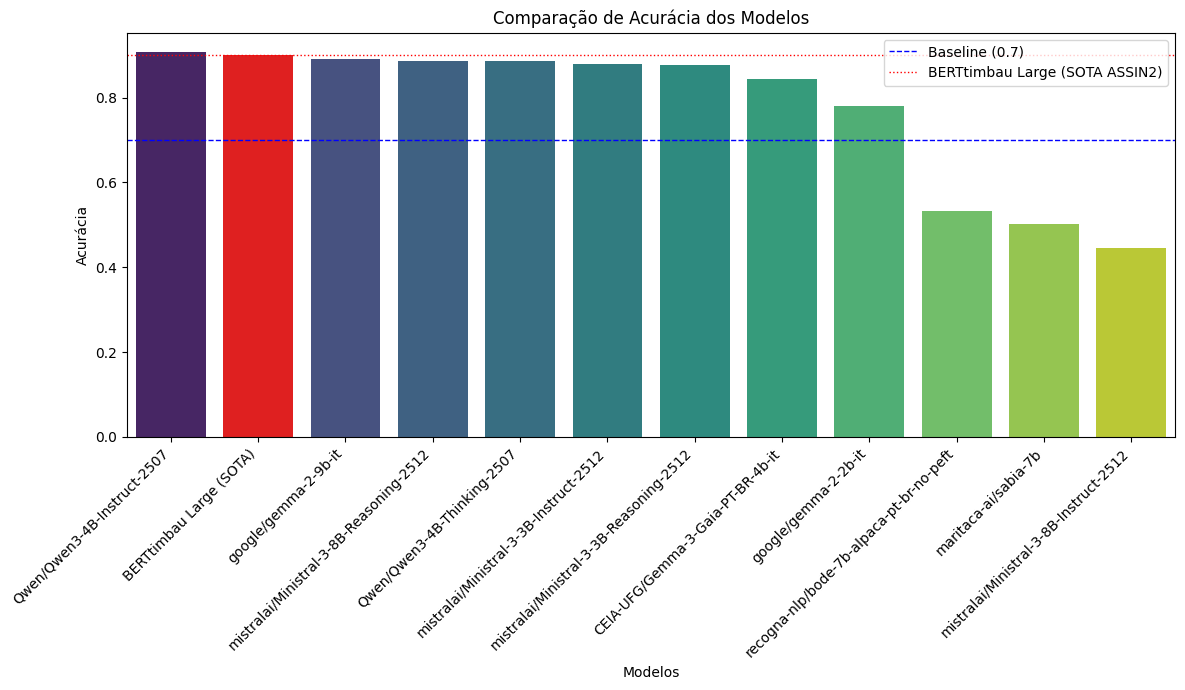
\includegraphics[width=0.90\textwidth]{figuras/grafico_acuracia_geral.png}
    \caption{Acurácia global no ASSIN~2. Linha tracejada: piso heurístico
    (0,70); linha pontilhada: teto supervisionado BERTimbau-large (0,90).}
    \label{fig:accuracy_assin2}
\end{figure}

Modelos multilíngues recentes lideram: o Qwen3-4B-Instruct atinge 90,8\%,
equiparando-se ao teto supervisionado em regime \emph{zero-shot}. O Gemma-2-9B
e variantes \emph{Reasoning} do Ministral também superam 87\%. Modelos
especializados em português exibem comportamento heterogêneo: o Gaia alcança
84,4\%, mas Sabiá-7B e Bode-7B sofrem colapso de classe (acurácia global
$\approx$~50\%, equivalente ao acaso).

\subsection{ASSIN~2: acurácia por classe}

A Tabela~\ref{tab:assin2} desagrega as acurácias por tipo de julgamento.
Observa-se assimetria recorrente: a maioria dos modelos erra mais na classe
\emph{Não Acarretamento}, tendendo a aceitar hipóteses que não são formalmente
acarretadas pela premissa. Sabiá-7B e Ministral-8B-Instruct colapsam para a
classe negativa (0,0\% e 0,7\% em acarretamento); Bode-7B colapsa para a
positiva (99,9\% em acarretamento, 7,2\% em não-acarretamento).

\begin{table}[ht]
\centering
\caption{Acurácia (\%) por tipo de julgamento no ASSIN~2.}
\label{tab:assin2}
\begin{tabular}{lccc}
\toprule
\textbf{Modelo} & \textbf{Acarretamento} & \textbf{Não Acarret.} & \textbf{Global} \\
\midrule
Qwen3-4B-Instruct            & 94,7 & 86,8  & \textbf{90,8} \\
Gemma-2-9B-IT                & 91,2 & 87,0  & 89,0 \\
Ministral-8B-Reasoning       & 93,9 & 83,6  & 88,7 \\
Qwen3-4B-Thinking            & 96,3 & 80,9  & 88,6 \\
Ministral-3B-Instruct (FP8)  & 89,9 & 86,0  & 88,0 \\
Ministral-3B-Reasoning       & 85,4 & 90,3  & 87,8 \\
Gemma-3-Gaia-PT-BR-4B        & 95,9 & 72,9  & 84,4 \\
Gemma-2-2B-IT                & 95,2 & 60,9  & 78,0 \\
Bode-7B                      & 99,9 & 7,2   & 53,4 \\
Sabiá-7B                     & 0,0  & 100,0 & 50,2 \\
Ministral-8B-Instruct (FP8)  & 0,7  & 87,7  & 44,5 \\
\bottomrule
\end{tabular}
\end{table}

\subsection{ASSIN~2: acurácia por faixa de similaridade semântica}

A Tabela~\ref{tab:catsim} apresenta a acurácia segmentada pelas faixas de
similaridade semântica (escala STS do ASSIN~2, de 1 a 5). Conforme definido
por~\cite{real2020assin}, o valor 1 representa sentenças ``totalmente
diferentes'' e o valor 5, ``significado virtualmente idêntico''.

\begin{table}[htbp]
\centering
\caption{Acurácia (\%) por faixa de similaridade semântica (ASSIN~2).}
\label{tab:catsim}
\begin{tabular}{lcccccc}
\toprule
\textbf{Modelo} & \textbf{1--2} & \textbf{2--3} & \textbf{3--4} & \textbf{4--5}
                & \textbf{5} & \textbf{Global} \\
\midrule
Qwen3-4B-Instruct      & 98,5  & 93,3 & 92,4 & 88,3 & 91,3 & 90,8 \\
Gemma-2-9B-IT          & 97,5  & 95,5 & 90,7 & 86,7 & 89,2 & 89,1 \\
Ministral-8B-Reas.     & 94,9  & 91,7 & 89,3 & 85,7 & 89,9 & 88,7 \\
Qwen3-4B-Thinking      & 99,5  & 96,2 & 91,2 & 83,5 & 89,9 & 88,6 \\
Minist.-3B-Instr.(FP8) & 95,5  & 95,7 & 90,8 & 85,5 & 87,8 & 88,0 \\
Minist.-3B-Reas.       & 93,4  & 94,0 & 93,0 & 88,3 & 85,5 & 87,8 \\
Gaia-PT-BR-4B          & 100,0 & 95,7 & 82,3 & 75,3 & 88,7 & 84,4 \\
Gemma-2-2B-IT          & 98,5  & 82,6 & 69,3 & 65,9 & 86,3 & 78,0 \\
Bode-7B                & 10,1  & 6,4  & 7,3  & 27,9 & 86,5 & 53,4 \\
Sabiá-7B               & 100,0 & 99,8 & 97,6 & 78,9 & 14,3 & 50,2 \\
Minist.-8B-Instr.(FP8) & 95,5  & 94,3 & 86,5 & 67,3 & 13,4 & 44,5 \\
\bottomrule
\end{tabular}
\end{table}

Nas faixas 1--2 (sentenças totalmente distintas), os melhores modelos atingem
acurácia próxima de 100\%, pois a decisão de não-acarretamento é trivial: a
dissimilaridade total torna a relação dedutiva evidentemente falsa. O desafio
intensifica-se nas faixas 3--4 e 4--5, onde a alta sobreposição lexical pode
induzir modelos dependentes de similaridade a classificar incorretamente pares
de alta semelhança como acarretamentos, mesmo quando a relação lógica não se
sustenta.

O fenômeno mais crítico ocorre na faixa~5 (paráfrases): Sabiá-7B (14,3\%) e
Ministral-8B-Instruct (13,4\%) colapsam justamente quando as sentenças são
virtualmente idênticas, revelando viés sistemático pela classe negativa. O
Bode-7B exibe o padrão inverso: acerta bem na faixa~5 (86,5\%) mas colapsa nas
faixas~1--2 (10,1\%), associando diretamente sobreposição lexical a
acarretamento.

\subsection{Dataset sintético: robustez sob controle semântico}

A Figura~\ref{fig:accuracy_sintetico} e a Tabela~\ref{tab:sintetico} apresentam
os resultados no dataset sintético, construído exclusivamente com pares baseados
em hiponímia.

\begin{figure}[htbp]
    \centering
    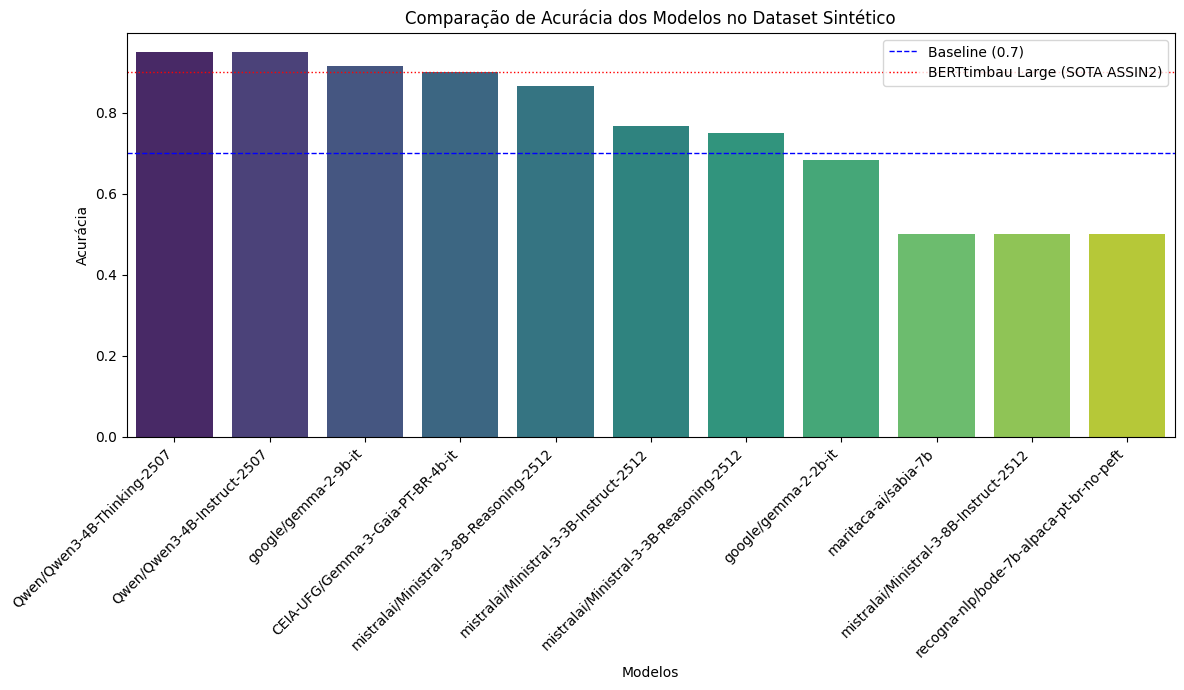
\includegraphics[width=0.90\textwidth]{figuras/grafico_acuracia_dados_sinteticos.png}
    \caption{Acurácia global nos dados sintéticos. Linhas de referência iguais
    às da Figura~\ref{fig:accuracy_assin2}.}
    \label{fig:accuracy_sintetico}
\end{figure}

\begin{table}[htbp]
\centering
\caption{Acurácia (\%) por tipo de julgamento no \emph{dataset} sintético.}
\label{tab:sintetico}
\begin{tabular}{lccc}
\toprule
\textbf{Modelo} & \textbf{Acarretamento} & \textbf{Não Acarret.} & \textbf{Global} \\
\midrule
Qwen3-4B-Thinking            & 90,0  & 100,0 & \textbf{95,0} \\
Qwen3-4B-Instruct            & 90,0  & 100,0 & \textbf{95,0} \\
Gemma-2-9B-IT                & 83,3  & 100,0 & 91,7 \\
Gemma-3-Gaia-PT-BR-4B        & 90,0  & 90,0  & 90,0 \\
Ministral-8B-Reasoning       & 73,3  & 100,0 & 86,7 \\
Ministral-3B-Instruct (FP8)  & 53,3  & 100,0 & 76,7 \\
Ministral-3B-Reasoning       & 50,0  & 100,0 & 75,0 \\
Gemma-2-2B-IT                & 96,7  & 40,0  & 68,3 \\
Bode-7B                      & 100,0 & 0,0   & 50,0 \\
Ministral-8B-Instruct (FP8)  & 0,0   & 100,0 & 50,0 \\
Sabiá-7B                     & 0,0   & 100,0 & 50,0 \\
\bottomrule
\end{tabular}
\end{table}

Qwen3-4B (\emph{Instruct} e \emph{Thinking}) e Gemma-2-9B mantêm acurácia
$\geq$91,7\%, demonstrando capacidade de generalização para a relação hiponímica
sem dependência de regularidades do ASSIN~2. O Gaia também exibe robustez
(90,0\%), sugerindo que a especialização em português é mais eficaz quando
combinada com uma base sólida de raciocínio. Em contraste, Sabiá, Bode e
Ministral-8B-Instruct preservam o padrão de colapso, atingindo apenas 50\%,
acaso puro, em pares construídos para isolar a relação semântica formal.

\subsection{Discussão}

\textbf{Dedução \emph{vs.} indução nos modelos.}\ A tipologia de Peirce oferece
uma moldura interpretativa para os comportamentos observados. Modelos que
colapsam para uma classe, Sabiá (sempre ``não acarreta''), Bode (sempre
``acarreta''), Ministral-8B-Instruct (sempre ``não acarreta''), evidenciam
que o processo indutivo de treinamento não se converteu em capacidade dedutiva
estável. Esses modelos não verificam as condições de verdade da relação entre
premissa e hipótese: operam como classificadores de similaridade global,
usando a distribuição léxico-semântica como \emph{proxy} para a decisão
inferencial. Esse comportamento reproduz as mesmas limitações das heurísticas
simbólicas identificadas por~\cite{stil}: a distinção entre similaridade
distribucional e preservação de condições de verdade permanece opaca para
modelos sem mecanismos explícitos de raciocínio.

\textbf{Raciocínio explícito como aproximação à dedução.}\ Os melhores modelos, Qwen3, Gemma~2 e variantes \emph{Reasoning} do Ministral, exibem
comportamento mais consistente com a estrutura dedutiva da tarefa: mantêm alto
desempenho tanto nas faixas de baixa similaridade (rejeição correta de pares
dissimilares) quanto na faixa~5 (aceitação correta de paráfrases), e preservam
essa robustez nos dados sintéticos. A \emph{Chain-of-Thought} e a destilação de
conhecimento parecem funcionar como mecanismos que aproximam o comportamento
indutivo dos modelos da verificação lógica de condições de verdade.

A comparação entre Qwen3-4B-Thinking (88,6\% no ASSIN~2 e 95,0\% no sintético)
e Qwen3-4B-Instruct (90,8\% e 95,0\%) indica que o \emph{thinking mode}, embora
marginalmente inferior no \emph{benchmark}, é igualmente robusto em dados
controlados. A superioridade do modo \emph{instruct} no ASSIN~2 pode refletir
uma exploração mais eficiente de padrões superficiais do \emph{benchmark}, e não
necessariamente maior competência inferencial estrita.

\textbf{A anomalia do Ministral-8B-Instruct.}\ A disparidade entre
Ministral-3B-Instruct (88,0\%) e Ministral-8B-Instruct (44,5\%) é
contra-intuitiva perante as leis de escala. A análise sugere que o alinhamento
ODPO no modelo de 8B, ao otimizar concisão e segurança para assistentes de
\emph{chat}, suprimiu a capacidade de raciocínio inferencial explícito. A
destilação de \emph{logits} específica aplicada ao modelo de 3B, combinada com
a arquitetura de \emph{tied embeddings}, mitigou esse efeito. O resultado indica
que o alinhamento para fluência conversacional pode ser prejudicial à verificação
lógica quando não acompanhado de cadeia de pensamento.

\textbf{\emph{Zero-shot} \emph{vs.} supervisionado.}\ O Qwen3-4B-Instruct
(90,8\%) iguala o BERTimbau-large ajustado supervisionadamente no ASSIN~2
(0,90), sem qualquer exemplo de treinamento. Isso demonstra que LLMs modernos
compactos conseguem atingir o teto do estado da arte supervisionado, eliminando
o custo de anotação manual. A diferença reside no custo de inferência: o
BERTimbau-large opera com $\sim$335M parâmetros e pode rodar em hardware de
entrada; o Qwen3-4B, mesmo quantizado, exige GPUs de pelo menos 8GB de VRAM.
Para cenários de prototipagem rápida ou escassez de dados anotados, os LLMs
\emph{zero-shot} oferecem, portanto, uma alternativa viável ao ciclo custo-
oso de anotação e treinamento supervisionado.

\section{Conclusão}

Este trabalho avaliou comparativamente 11 LLMs compactos em NLI em português
brasileiro, em regime estritamente \emph{zero-shot}, contrastando especialização
linguística e raciocínio explícito. A introdução de um \emph{dataset} sintético
baseado em acarretamento por inclusão lexical (hiponímia/hiperonímia), alinhado
à definição formal de~\cite{Ferreira2019}, permitiu separar competência
inferencial genuína da exploração de regularidades superficiais do
\emph{benchmark}.

Os resultados indicam que raciocínio explícito e destilação de conhecimento são
mais decisivos do que adaptação monolíngue isolada para a tarefa. Do ponto de
vista da semântica formal, modelos que exibem colapso de classe estão
substituindo a verificação dedutiva de condições de verdade, a relação que
define o acarretamento~\cite{Ferreira2019}, pelo reconhecimento indutivo de
similaridade distribucional. Acurácia elevada no ASSIN~2 pode, portanto,
superestimar a competência inferencial quando não verificada em dados construídos
sob restrição semântica estrita.

Como trabalhos futuros, vislumbra-se a extensão do dataset sintético para outros
fenômenos da semântica formal além da inclusão lexical, como acarretamento por
predicação e por operadores modais, e a avaliação em regime \emph{few-shot}
para quantificar o ganho decorrente de exemplos explícitos.

\bibliographystyle{sbc}
\bibliography{refs}

\end{document}
